\documentclass[12pt]{article}

\usepackage{color}
\usepackage[dvipsnames]{xcolor}
\usepackage{listings}
\usepackage{graphicx}


%for linkt page numbers in table of content
\usepackage[linktocpage=true]{hyperref}

\hypersetup{%
unicode,pdffitwindow,
pdfkeywords = {pdf, LaTeX, hyperref, thumbnails}, 
pdfauthor = {Brüder Grimm},
bookmarksopen = true,
bookmarksnumbered = true,
pdfcenterwindow=true,
pdffitwindow = true,
pdfstartview=FitBV,
pdfcreator = {pdflatex},
colorlinks=true, breaklinks=true, %
urlcolor=magenta, % color for \url
filecolor=cyan, % color for file
linkcolor=black, % color for \ref
citecolor=magenta, %color for \cite
menucolor=darkblue,
breaklinks=true,anchorcolor=green
}
\usepackage{caption}
\DeclareCaptionFont{white}{\color{white}}
\DeclareCaptionFormat{listing}{\colorbox{teal}{\parbox{\textwidth}{#1#2#3}}}
\captionsetup[lstlisting]{format=listing,labelfont=white,textfont=white}

\definecolor{dkgreen}{rgb}{0,0.6,0}
\definecolor{gray}{rgb}{0.5,0.5,0.5}
\definecolor{mauve}{rgb}{0.58,0,0.82}
\colorlet{LightRubineRed}{red!30!orange!30}  %30%red with 70%orange and this collor mixed with 70% withe

\lstset{
  language=Java,
  basicstyle=\small,
  numberstyle=\tiny\color{gray},
  keywordstyle=\color{blue},
  commentstyle=\color{dkgreen},
  stringstyle=\color{mauve},
  lineskip=0pt,
  backgroundcolor=\color{LightRubineRed}
}

% This concludes the preamble
\usepackage{setspace}
\linespread{1.25}

%for geometry
\usepackage{geometry}
\geometry{ headsep=20pt,
headheight=20pt,
left=21mm,
top=15mm,
right=21mm,
bottom=15mm,
footskip=20pt,
includeheadfoot}
% no paragraph indent
\setlength{\parindent}{0em}

%for geometry

%-----------------------------------------------------
\title{Java Uni ab Woche 7}
\begin{document}

\maketitle
\tableofcontents

\addcontentsline{toc}{section}{Datentypen und Objekte}
\section*{Datentypen und Objekte}
Etwas abstrakt formuliert ist ein Datentyp, ein Menge von Werten, zusammen mit Operationen die auf diese Werten definiert
sind. Jeder Wert in Java ist also eine Instanz eines Bestimmten Datentyps.

Operationen sind zum beispiel bei \textbf{int} die addition oder bei \textit{arrays} die [] um auf elemte zu zugreifen. 

Um eine Instanz eines Datentyps zu erstellen benutzen wir das Schlüsselwort new. 


    \begin{lstlisting}[label=some-code,caption=Erzeugung Instanz]
// Erzeugen eines Werts des Datentyp Strings
String s = new String("hello world");
    \end{lstlisting}


    Operationen auf eine Wert werden imttels Methodenaufrufung ausgeführt

    \begin{lstlisting}[label=some-code,caption=Erzeugung Instanz]
// Anwenden der Operation lenght auf dem Wert "hello world"
s.lenght();
    \end{lstlisting}

    In der Objektorientierten Programmierung werden Instanzen oder Werte von Datentypen \textbf{Objekte} gennant. 
    Die variable \textbf{s} aus dem beispiel \textbf{referenziert} das Objekt \textit{String}. 

    Die Primitiven Datentypen (int, double, cahr, etc.) haben eine Wrappenklasse um sie auch wie andere Objekte behandeln zu können. 

    \begin{table}[h]
        \centering
        \begin{tabular}{| c | c | }
            \hline
            Primitiver Datentyp & Wrapper \\
            \hline
            int & Integer \\
            \hline
            double & Double \\
            \hline 
            boolean & Boolean \\
            \hline 
            char & Character \\
            \hline 
            float & Floar \\
            \hline 
            short & Short \\
            \hline 
            long & Long \\
            \hline 
            byte & Byte \\
            \hline 
            

        \end{tabular}
    \end{table}


\section*{Objektorientierung}
\addcontentsline{toc}{section}{Objektorientierung}
    Funktionen verwenden wir um Sequenzen von Anwesungen zu abstrahieren.
    Ähnlich dazu werden wir nun Klassen verwenden um zusammengehörige Daten zu einer grösseren Einheit zusammenzufassen. 
    Werte dieser Klassen (also Instanzen der Datentypen) werden Objekte genannt. 
    Diese Art der Datenorganisation mittels Klassen führt zu einer Art der Softwareentwicklung, die sich Objektorientierte Programmierung nennt.

    \subsection*{Klassen}
    \addcontentsline{toc}{subsection}{Klassen}
    Klassen sind ein Konstrukt mit dem wir Datentypen definieren können. Dafür müssen wir die Werte, welche repräsentiert weden, definieren und 
    Operationen welche auf diesen Werten ausgeführt werden können. 

        \subsubsection*{Definition der Klasse}
        \addcontentsline{toc}{subsubsection}{Definition und Klassen}
        Um eine Klasse zu definieren müssen wir das Schlüsselwort \textbf{class} benutzen. Ein beispiel. 

        \begin{lstlisting}[label=Klassen definieren,caption=Klasse definieren]
            class Point {

            }
        \end{lstlisting}

        \subsubsection*{Felder der Klassen}
        \addcontentsline{toc}{subsubsection}{Felder der Klassen}

        Die Daten die unser Datentyp repräsentiert nennen wir \textbf{Felder} oder \textit{Attribute}. Diese definieren wir einfach 
        inerhalt der Klassenrumpfs. In diesem beispiel hat ein Punkt x und y Koordinate, welche wir verwenden und repräsentieren wollen. 

        \begin{lstlisting}[label="", caption=Felder]
            class Point {
                double x;
                double y;
            }
        \end{lstlisting}

        \subsubsection*{Erzeugen von Objekten}
        \addcontentsline{toc}{subsubsection}{Erzeugen von Objekten}
        Im Folgenden beispiel erzeugen wir zwei Instanzen des Datentyps \textbf{Point} und weisen diese den Vatiablen \textit{point1} un d\textit{point2} zu.

        \begin{lstlisting}[caption=Erzeugen von Objekten]
            Point point1 = new Point();
            Point point2 = new Point();
        \end{lstlisting}


        \subsubsection*{Setzen und Lesen der Werte der Felder eines Objekts}
        \addcontentsline{toc}{subsubsection}{Setzen und Lesen der Werte der Felder eines Objekts}

        Wir wollen point1 die Koordinaten $(0,0)$ und point2 $(1,2)$ zuweisen.

        \begin{lstlisting}[caption=zuweisen von Werten auf Felder]
            point1.x = 0;
            point1.y = 0;

            point2.x = 1;
            point2.y = 2;
        \end{lstlisting}

        \begin{lstlisting}[caption=ausgeben der Werte]
    System.out.println("point1, x-koordinate:" + point1.x);
    //...
        \end{lstlisting}

        \subsubsection*{Methoden}
        \addcontentsline{toc}{subsubsection}{Methoden}

        Der zweite Teil einer Definition eines Datentyps sind die Operationen, die wir darauf ausführen können. 
        Diese werden über Methoden definiert.

        Methode um Punkt um \textbf{dx} und \textbf{dy} zu verschieben

        \begin{lstlisting}[caption=methode]
        class Point {
                double x; 
                double y;

            public void translate(double dx, double dy) {
                x = x + dx;
                y = y + dy;
            }
        }
        \end{lstlisting}

        Die methode nimmt als Paramater zwei Gleitkommazahlen entgegen und addiert sie zu den 
        bestehenden Variablen hinzu das kann sie weil sie auf diese Zugreifen kann. 


        \begin{lstlisting}[caption=ausführen methode]
    p1.translate(2, 3); // Translates object p1 of type Point
        \end{lstlisting}

        \subsubsection*{Konstruktor}
        \addcontentsline{toc}{subsubsection}{Konstruktor}

        Um Werte einem Objekt direkt beim erstellen zu übergeben nutzen wir eine Konstruktor. Dieser muss 
        gleich heissen wie die Klasse. 

        \begin{lstlisting}[caption=Konstruktor]
        class Point {
            double x;
            double y;

            // Definition des Konstruktors
            Point(double xValue, double yValue) {
                x = xValue;
                y = yValue;
            }
        }
        \end{lstlisting}

        \begin{lstlisting}[caption=nutzen Konstruktor]
            Point p1 = new Point(0, 0);
        \end{lstlisting}


        \subsubsection*{Klassen sind Referenzdatentypen}
        \addcontentsline{toc}{subsubsection}{Klassen sind Referenzdatentypen}
        Eine Variable eines Referenzdatentyps ist nur eine Adresse des eigentlcihen typs. Heisst wir können nicht einfach zwei Objekte gleich setzen und der eine 
        Typ wrid dem anderen übergene. 

        Um Variabeln der Felder genau anzusprechen könne wird das Schlüsselwort \textbf{this} vor diese Variabeln setzen.

        \subsubsection*{Klassenfelder und Klassenmethoden}
        \addcontentsline{toc}{subsubsection}{Klassen und Klassenmethoden}

    Java unterscheidet Felder wie auch Methoden ob sich diese auf ein Objekt oder eine Klasse beziehen. 
    Wir sprechen dann jeweils von Objektfelder/Objektmethoden und Klassenfelder/Klassenmethoden. 
    Dabei brauchen wir für Objektfelder/Objektmethoden ein Objekt um auf diese zuzugreifen oder diese aufzurufen. 
    Bei den Klassenfeldern/Klassenmethoden verwenden wir stattdessen die Klasse durch deren Klassennamen.

    static vor einer Methode oder Feld, heisst diese können genutzt werden ohne Instanz der Klasse erstellt zu haben. 

\section*{Objektorientierung 2}
\addcontentsline{toc}{section}{Objektorientierung 2}

In diesem Abschnitt werden wir Konsepte kennenlernen welche uns ermöglichen Hierarchien zu erstellen und wir werden Interfaces kennenlernen,
mit welchen wir die Operationen eines Datentyps von der Implementation trennen können. Somit können wir Schnittschtelle zwischen verschiedenen Implementation 
erstellen. 

    \subsection*{Interfaces}
    \addcontentsline{toc}{subsection}{Interfaces}

    Ein Interface gibt uns die Möglichkeit die Operationen einer Klasse von der Implementation dieser Operationen zu trennen. 
    Ein Interface spezifiziert einfach eine Menge von Methoden, die ein Datentyp zur Verfügung stellen muss.

    Wir zeigen an einem Beispiel den Nutzen der Interfaces. 
    Wir wollen eine Anwendung programmierung welche geometrische Elemente zeichnen können soll. Diese Elemente (Kreise, Dreiecke, Rechtecke etc.) 
    sollen auch manipuliert, vergössert, verkleinert und verschoben werden könne. 


    Um die Objekte zu skalieren, definieren wir auf jedem Datentypen die Methode \textbf{scale(double scaleFactor)} 

    \begin{lstlisting}[caption=Scalable]
interface Scalable {
    void scale(double scaleFactor); // Methodensignatur 
}
    \end{lstlisting}

    Wir definieren uns ein zweites Interface, welche die Methoden für das Positionieren des Objekts zur Verfügung stellt:

    \begin{lstlisting}[caption=Movable]
interface Movable {
    void translate(double x, double y);
    void moveToOrigin();
}
    \end{lstlisting}

    Wenn wir die geometrischen Objekte implementieren könne wir bestimmen welche Interfaces sie unterstützen. 
    Wir sprechen davon, dass eine Klasse ein Interface implementiert. Tatsächlich wird jedoch nicht das Interface implementiert, 
    sondern die im Interface definierten Methoden.

    Im Folgenden finden Sie die Beispieldefinition einer Klasse Circle. 
    Diese implementiert die in den Interfaces Movable und Scalable definierten Methoden.


    \begin{lstlisting}[caption=Circle]
class Circle implements Movable, Scalable {
    double xPos;
    double yPos;
    double radius;

    public void translate(double x, double y) {
        this.xPos = this.xPos + x;
        this.yPos = this.yPos + y;
    }

    public void moveToOrigin() {
        this.xPos = 0;
        this.yPos = 0;
    }

    public void scale(double scaleFactor) {
        this.radius = this.radius * scaleFactor;
    }
}
    \end{lstlisting}

    Nach dem Schlüsselwort \textbf{implements} werden die Interfaces angegeben die implementieren werden sollen. 
    Die Methoden müssen im Klassenrumpf definiert und implementiert werde, ebenso müssen sie \textbf{public} sein. 

    Nicht alle Elemente in unserer Anwendung müssen skalierbar sein. So zum beispiel der Datentyp \textbf{Point} welcher nur \textbf{Movable} implementieren muss. 

    \begin{lstlisting}[caption=Point]
        class Point implements Movable {
            double xPos;
            double yPos;

            public void translate(double x, double y) {
                this.xPos = this.xPos + x;
                this.yPos = this.yPos + y;
            }

            public void moveToOrigin() {
                this.xPos = 0;
                this.yPos = 0;
            }

        }
    \end{lstlisting}

    Die Klassen Point und Circle haben nun also beide das Interface Moveable implementiert. Davon können wir in unserer Anwendung Gebrauch machen. 
    Wir können Methoden schreiben, welche für ein Objekt nur ein Interface voraussetzen und benutzen. 
    Es müssen dann lediglich die in einem spezifizierten Interface definierten Methoden implementiert sein. 
    Es wird jedoch nicht einen konkreter Datentyp verlangt.

    Wir können also eine Methode schreiben ohne genau angeben zu müssen von Welchem Datentyp die Methode verwenden will. 

    \begin{lstlisting}[caption=moveAround]
public static void moveAround(Movable m, double xv, double yv) {
    m.translate(xv, yv);
}
    \end{lstlisting}

    Beachten Sie, dass wir hier statt des Datentyps Circle oder Point einfach den Namen des Interface Movable verwendet haben. 
    Dadurch weiss Java, dass die Methode translate zur Verfügung steht.

    \begin{lstlisting}[caption=verschieben Objekte]
Circle aCircle = new Circle();
Point aPoint = new Point();

moveAround(aCircle, 10, 20);
moveAround(aPoint, 0, 1);
    \end{lstlisting}

    Wir können auch direkt Variablen vom Typ des Interfaces definieren. 

    \begin{lstlisting}[caption=Interface nutzung]
Movable movable1 = new Circle();
Movable movable2 = new Point();
    \end{lstlisting}

    \subsection*{Vererbung und abstrakte Klassen}
    \addcontentsline{toc}{subsection}{Vererbung und abstrakte Klassen}

    Mittels Interfaces könne wir Datentypen erstellen welche gleiche Fähigkeiten haben müssen
    aber sonst nicht miteinander zu tu haben. 

    Mit hilfe der Vererbung können wir Hierarchien erstellen. Wir können Konzepte erstellen, welche spezifischere Konzepte andere Konzepte sind. 
    Zum beispiel sind Bannane ein Unterkonzept der Frucht. 

    Solche Hierarchien könne wir mir Abstrakten Klassen erstellen. Diese werden gleich wie andere Klassen definiert nur mit dem Schlüsselwort \textbf{abstract} 

    \begin{lstlisting}[caption=abstrakte Klasse]
abstract class Fruit {
    String name;
    String color;

    public Fruit(String name, String color) {
        this.name = name;
        this.color = color;
    }
    
    void eat() { System.out.println("eat"); }
}
    \end{lstlisting}

    Abstrakte Klassen können das gleiche wie "normale" Klassen. \textbf{Von Abstrakten Klassen könne keine
    Instanzen erstellt werden. }
    Mittels abstrakter Klassen wird nur das allgemeine Konzept definiert, welches dann von konkreten, spezialisierten Klassen umgesetzt wird.


    \begin{lstlisting}[caption=Fruit]
class Banana extends Fruit {

    public Banana() {
        super("Banana", "yellow");
    }
}
    \end{lstlisting}

    Das Schlüsselwort \textbf{extends} zeigt das die Klasse \textbf{Banana} von \textbf{Fruit} erbt. 
    Die vererbende Klasse wird auch \textbf{Superklasse} gennant. 
    Im Konstruktor der Klasse Banana, müssen wir als erste Anweisung den Konstruktor der Superklasse aufrufen. Dazu verwenden wir das Schlüsselwort \textbf{super}.
    Da Banana von Fruit erbt, müssen alle Eigenschaften, die für das allgemeine Konzept Fruit gelten, auch für die konkrete Spezialisierung Banana gelten. 
    Wir können entsprechend auf Instanzen vom Typ Banana auf alle Methoden und Felder von Fruit zugreifen.

    \begin{lstlisting}[caption=Beispiel Superklasse]
abstract class Fruit {
    String name;
    String color;

    public Fruit(String name, String color) {
        this.name = name;
        this.color = color;
    }
    
    void eat() { System.out.println("eat"); }
}

class Banana extends Fruit {

    public Banana() {
        super("Banana", "yellow");
    }
}

class AbstractClassExperiment {
  
  public static void main(String[] args) {
    Banana aBanana = new Banana();
    aBanana.eat();
    System.out.println(aBanana.color);
  }
}
    \end{lstlisting}


    Genau wie bei Interfaces, ist es auch in abstrakten Klassen möglich, Methoden nur zu deklarieren, nicht aber zu implementieren.
    Dies macht Sinn, da im abstrakten Konzept ja gewisse Verhalten noch unklar sein können, und nur in den konkreten Klassen wohldefiniert sind. 
    In unserem Frucht-Beispiel könnten wir in der Abstrakten Klasse Fruit eine Methode prepare definieren. 
    Diese soll beschreiben, wie eine Frucht zubereitet werden kann. 
    Wie diese aber umgesetzt werden soll, hängt von der konkreten Frucht ab. 
    Nicht jede Frucht wird gleich zubereitet. 
    In Java können wir dies wie folgt umsetzten:

    \begin{lstlisting}[caption=abstrakte Methoden]
abstract class Fruit {
    String name;
    String color;

    public Fruit(String name, String color) {
        this.name = name;
        this.color = color;
    }

    abstract void prepare();
}

class Banana extends Fruit {

    public Banana() {
        super("Banana", "yellow");
    }

    void prepare() {
        System.out.println("peel");
        System.out.println("eat");
    }
}

class Mango extends Fruit {

    public Mango(String color) {
        super("Mango", color);
    }

    void prepare() {
        System.out.println("peel");
        System.out.println("slice");        
        System.out.println("eat");
    }
}
    \end{lstlisting}

    \subsection*{Polymorphismus und Dynamische Bindung}
    
    Bei Polymorphismus handelt sich um das Nutzen von Subklassen ohne diese genau 
    anzusprechen. Zu beispeil wenn die Klasse \textbf{Banana} die abstrakte Klasse 
    \textbf{Fruit} extends und wir in einer Methode als Parameter \textbf{Fruit} angeben 
    aber diese Methode auch eine Instanz von \textbf{Banana} entgegen nehmen kann. 

    Die idee von Dynamischer Bindung ist, dass wenn wir in einem Interface oder einer 
    abstrakten Klasse eine Methode definieren und diese denn auf Subklassen implementieren, 
    wir diese Flexibel einsetzen können. Wenn wir eine Methode schreiben die dann z.b 
    \textbf{Fruit} entgegen nimmt und \textbf{prepare()} auf \textbf{Banana} und \textbf{Mango}
    definiert sind. Könne wir \textbf{prepare} auf Fruit anwenden, obwohl sie dort nicht
    implementiert ist und dann wird sie so ausgeführt abhengig davon was der Ursprünglischen 
    Methode gegeben wird. Ob eine Instanz von \textbf{Mango} oder \textbf{Banana}. Hier der 
    Code dazu 

    \begin{lstlisting}[caption=Polymorphismus]
abstract class Fruit {

    abstract void prepare();
  
}

class Banana extends Fruit {

    void prepare() {
        System.out.println("peel");
        System.out.println("eat");
    }
}

class Mango extends Fruit {

    void prepare() {
        System.out.println("peel");
        System.out.println("cut");
        System.out.println("eat");
    }

}

class FruitExample {

    static void preparationInstructions(Fruit aFruit) {
        aFruit.prepare(); // abhaengig von input in Methode
    }

    public static void main(String[] args) {
        Banana aBanana = new Banana();
        Mango aMango = new Mango();

        preparationInstructions(aBanana);
    }
}
    \end{lstlisting}

    \subsection*{Klassenhierarchie}

    Java ist in einer Hierarchie aufgebaut. Und ganz oben ist der Datentyp \textbf{Object}. Jede neue Klasse erbt von diesem Typ. 
    In dem Datentyp \textbf{Object} werden wichtige Methoden definiert welche auf jedem objekt verwendet werden können. 
    Es gitb weitere Hierarchien wie das \textbf{Integer} von \textbf{Number} erbt. 


    \subsubsection*{Downcasting}

    Wir könne also in eine Variable vom Tyo \textbf{Object} eine Instanz vom Typ Integer machen, weil \textbf{Object} ganz obe in der Hierarchie ist. 

    \begin{lstlisting}[caption=erbt von Object]
Object anInteger = new Integer(5);
Object aString = new String("Hello world");
    \end{lstlisting}

    Umgekehrt geht das aber nicht, da java nicht garantieren kann, das beim zurück welchseln nicht ein andere Wert eingesetzt wurde der nicht 
    eine Subklasse der spezifischen Superklasse ist. 

    \begin{lstlisting}[caption=fehler]
Object anInteger = new Integer(5);
Integer theSameInterger = anInteger; // Fehler
    \end{lstlisting}

    Wir könne java aber dazu zwingen, dass es diesen prompt akzeptiert, indem wir das ganze casten. 

    \begin{lstlisting}[caption=casting]
Object anInteger = new Integer(5);
Integer theSameInterger = (Integer) anInteger; // Dies ist gueltig
    \end{lstlisting}

    Wenn jetzt aber \textbf{anInteger} nicht ein Integer ist gibt es einen 
    Laufzeitfehler. Wir können mit \textbf{instanceof} herrausfinden ob ein Object ein Subklasse von einem anderen Object ist. 
    Zum beispiel gibt \textbf{anInteger instanceof Integer} true aus. 

    \subsection*{Equals und toString}

    Die klasse \textbf{Object} definiert wichtige Methoden. Die zwei wichtigsten für diese 
    Zusammenzufassen ist \textbf{Equals und toString}. 

    Die Methode \textbf{toString} gibt uns die möglichkeit Objekte als String dar zu stellen. 
    Zum Beispiel ist 

    \begin{lstlisting}[caption=toString]
System.out.println(obj);
    \end{lstlisting}

    als \textbf{obj.toString } zu verstehen.

    In der Klasse \textbf{Object} wird die Methode \textbf{toString} zwar implementiert aber nur seht allgemein 
    da diese nicht viel über das Objekt weis an welchem die Methode ausgeführt wird. Es wird nur der Name der Klasse
    und eine interne Referenz ausgegeben. 
    Am beispiel der Point Klasse könne wir das gut sehen. 

    \begin{lstlisting}[caption=Point]
class Point {
    double x;
    double y;
    Point(double x, double y) {
        this.x = x;
        this.y = y;
    }
}
class ToString {
  public static void main(String[] args) {
    Point aPoint = new Point(3, 4);
    System.out.println(aPoint);
  }
}
    \end{lstlisting}

    Ausgabe: Point@6d06d69c
    
    Um eine sinvolle ausgabe zu mache müssen wir \textbf{toString} implementiere. Und dabei müssen wir die
    originale methode toString überschreiben und das machen wir mit dem Schlüsselwort \textbf{@Override}. 

    \begin{lstlisting}[caption=point]
class Point {
    double x;
    double y;
    Point(double x, double y) {
        this.x = x;
        this.y = y;
    }
    @Override
    public String toString() {
        return "(" +x + "," +y + ")";
    }
}
    \end{lstlisting}

    \subsection*{Die Equals Methode}

    Die Equals methode hat die Signatur: 

    \begin{lstlisting}[caption=Equals]
public boolean equals(Object obj) ;
    \end{lstlisting}

    Die Methode will das \textit{this} objekt mit dem Paramater objekt vergleiche. 
    Das machen wir so: 

    \begin{lstlisting}[caption=equals implementiert]
class Point {
    double x;
    double y;
    Point(double x, double y) {
        this.x = x;
        this.y = y;
    }
    @Override
    public boolean equals(Object obj) {

        if (!(obj instanceof Point))
            return false;
        else {
          Point other = (Point) obj;
          return this.x == other.x && this.y == other.y;
        }
    }
}
    \end{lstlisting}

\section*{Pakete, Module und Sichtbarkeit}

    Um den code besser zu strikturieren und die Wartbarkeit zu gewehrleisten, nutzen wir verschieden methoden. 
    Dies werden nachfolgend aufgeführt und erklärt. 

    \subsection*{Module und Information hiding}

    \href{https://unibas.cloud.panopto.eu/Panopto/Pages/Viewer.aspx?id=27c8490a-6428-452a-901e-af4e008d22f7&start=5.634217}{video}

    Um praktische Anwendungen zu programmieren müssen wir nicht immer die ganze Komplexität darstellen. 
    Für andere Mensche die unseren Code verwenden, nicht es nicht hilfreich die genau funktionsweise aller methoden zu kennen, 
    weshalb wir Code so strukturieren das wir nicht alles direkt erkennen könne. 

    Als beispielt gilt die autoschaltung. Wir können mit den Zahlen bei der Schaltung umgehen aber wissen 
    nicht genau was passiert wenn wir in de 2. Gang schalten. Und das müssen wir auch nicht. 

    \subsection*{Packages und Imports}

    Packages sind dazu da Klassen in Java zu ordnen. Dafür wird das Dateisystem genutzt. Zusammengehörende Klassen 
    müssen im gleichen Verzeichnis stehen. Der Name der Packages muss dem des Verzeichnisses entsprechen und muss in Quellcode vorhanden sein. 

    Angenommen wir haben drei Klassen A1, A2 und B1. Wir möchten, 
    dass die Klassen A1 und A2 Teil eines Packages mit dem Namen foo sind. 
    Die Klassen B soll ein Teil eines Packages mit dem Namen bar sein. 
    Wir hätten folgende Dateien und Verzeichnisse in unserem Projekt:

    \begin{lstlisting}[caption=packages]
./src/foo/A1.java
./src/foo/A2.java
./src/bar/B1.java
    \end{lstlisting}

    Der Quellcode sieht dann enstprechend aus. 

    \begin{lstlisting}[caption=quellcode]
package foo; // Paketdefintion, am Anfang der Datei

class A1 {
  // Implementation der Klasse
}
    \end{lstlisting}

    Hierarchien sind daruch auch möglich. Es können auch packages in packages verschatelt sein. das sieht dann so aus. 

    \begin{lstlisting}[caption=verschatelt packages]
./src/foo/A1.java
./src/foo/A2.java
./src/foo/sub1/A31.java
./src/foo/sub2/A41.java

package foo.sub1;

class A31 {
  // Implementation der Klasse
}
    \end{lstlisting}

    \subsection*{Packages als Namesräume}

    Durch die Anordnung in Packages haben wir den Klassen nun auch neue Namen gegeben. Die Klasse A1 im obigen Beispiel hat nun den vollen Namen foo.A1. 
    Die Klasse A31 hat den Namen foo.sub1.A31. Damit wird es möglich, denselben Klassennamen in verschiedenen Packages zu nutzen. 
    Durch den vollen Namen können diese voneinander unterschieden werden. In grossen Programmen, mit zehntausenden von Klassen, ist dies enorm wichtig. 
    Die Programmierer\*innen können sich auf das Paket konzentrieren, indem sie gerade arbeiten. 
    Sie können einen möglichst sinnvollen Klassennamen im aktuellen Paket wählen. 
    Es kommt zu keinen Problemen mit Namen von Klassen in anderen Packages.

    Dafür werden die Klassenname grösser. Beim nutzen sieht das jetzt so aus:

    \begin{lstlisting}[caption=klassen in packages]
package bar; 
class B1 {
    // Felder
    foo.sub1.A31 field1;
    foo.sub2.A32 field2;

    B1() {
      this.field1 = new foo.sub1.A31();
      this.field2 = = new foo.sub2.A32();
    }
}
    \end{lstlisting}

    Java vereinfacht die Klassennamen indem es: 

    \begin{itemize}

        \item annimt, wenn kein package angegeben ist, die Klasse im aktuellen Package vorhanden ist.

        \item Mit der Importklausel könne wir über kürzere namen verfügen

    \end{itemize}

    \subsection*{Importieren von Klassen}


    Um Klassen direkt ansprechen zu könne ohne noch den Packagenamen zu nutzen,
    müssen wir das Schlüsselwort \textbf{import} verwenden. 

    \begin{lstlisting}[caption=import Klassen]
package bar; 

import foo.sub1.A31;
import foo.sub2.A32;

class B1 {
    // Felder
    A31 field1;
    A32 field2;

    B1() {
      this.field1 = new A31();
      this.field2 = = new A32();
    }
}
    \end{lstlisting}

    Um alle Klassen eines Package zu importieren schreiben wir \textbf{*} ans ende des Package. 

    \subsection*{Bibliotheken in Java}

    Bibliotheken in java sind nichts weiteres als Sammlungen von Klassen, die in Packages strukturiert sind. Zum beispiel die 
    Klasse ArrayList. Sie zu importieren geht so:

    \begin{lstlisting}[caption=ArrayList]
import java.utils.ArrayList
    \end{lstlisting}


    \subsection*{Module}

    Wie bereits angemerkt bietet Java noch eine zusätzliche Funktionalität, um Programme zu organisieren. Diese werden Module genannt. 
    Jedes Modul beinhaltet eine Sammlung von Paketen. 
    Die oben gezeigten Pakete in der \href{https://docs.oracle.com/en/java/javase/17/docs/api/index.html}{API-Dokumentation} befinden sich alle im Module java.base. 
    Es gibt jedoch noch eine Vielzahl anderer Module. 
    Diese bestehen dann auch wieder aus dutzenden von Paketen mit hunderten von Klassen. 
    Welche Module in der aktuellen Java Version zur Verfügung stehen, können Sie auch in der Java API-Dokumentation nachschauen.

    Da Sie auf absehbare Zeit keine so grossen Programme schreiben werden und mit diesem Mechanismus auch nicht direkt in Berührung kommen werden, 
    werden wir Module in diesem Kurs nicht diskutieren.

    \subsection*{Zugriffsmodifikatoren}

    Für Klassen gibt es die Zugriffsmodifikatoren \textbf{public} und \textbf{default}.
    Um eine Klasse als public zu deklarieren schreiben wir einfach das Schlüsselwort public vor die Klasse:

    \begin{lstlisting}[caption=public]
public class AClass {}
    \end{lstlisting}

    Wenn keine angaben zum Zugriff gemacht werden. Wird von \textbf{default} ausgegange

    Das sind die Sichtbarkeitsregelen für Klassen
    \begin{table}[h]
        \centering
        \begin{tabular}{| c | c | }
            \hline
            Zugriffsmodifikator & Sichtbarkeit \\
            \hline
            public & Der Zugriff ist aus Klassen im Programm möglich. \\
            \hline
            default & Der Zugriff ist nur aus Klassen im selben Package möglich. \\
            \hline
        \end{tabular}
    \end{table}

    Wir deklarieren nur die wichtigen Klassen, die von aussen Sichtbar sein sollen als public. 
    Alle anderen Klassen, die nur der internen Implementation der Logik dienen, sind so vor den Benutzern versteckt. So 
    könne wir auch teile des Codes Ersetzten ohne mit anderem Code zu intervenieren. 

    \newpage
    \subsection*{Zugriffsmodifikatoren für Felder und Methoden}

    Für Felder und Methoden gibt es noch mehr Zugriffsmodifikatoren. Hier auch wenn nichts deklariert wird, 
    geht java von \textbf{default} aus. 


    \begin{table}[h]
        \centering
        \begin{tabular}{ | c | c |  }
            \hline
            Zugriffsmodifikator & Sichtbarkeit \\
            \hline
            public & Zugriff aus allen methoden möglich\\
            \hline 
            protected & Zugriff aus Methoden von selben Klassen, Package und aus Subklassen möglich. \\
            \hline 
            default & Der Zugriff ist nur aus Methoden von Klassen aus demselben Package möglich. \\
            \hline 
            private & Der Zugriff ist nur aus Methoden von derselben Klasse möglich \\
            \hline 

        \end{tabular}
    \end{table}

    Ein typisches Muster in der Objektorientierung ist es, die Felder alle als private zu deklarieren. Der Zugriff von Aussen wird nur über Methoden gewährt. 
    Die Idee dahinter ist, dass die Datenrepräsentation ein internes Detail ist und sich häufig ändern kann. 
    Im Gegensatz dazu wird das Verhalten, welches über die Methoden definiert ist, stabiler bleiben und sich weniger häufig ändern.

    \href{https://unibas.cloud.panopto.eu/Panopto/Pages/Viewer.aspx?id=bacffede-fd03-4d96-b1fb-af4e0095dfcd&start=6.708527}{genaue Funktionalitaet der Zugriffsmodifikatoren}

    \section*{Generics}

    \begin{lstlisting}
interface List<E> {
    // adds an Element to the list
    void add(E element);

    // returns the element at the given position
    E get(int index);
}
    \end{lstlisting}

    E steht für einen fixen Typen der aber noch nicht bekannt ist.

    \subsection*{Typparameter}

    \begin{lstlisting}
// Deklariert Variable vom Type List<String>
List<String> stringList;
    \end{lstlisting}

    Definieren einer Liste mit Strings als inhalt. 

    \begin{lstlisting}
List<Double> reverse(List<Double> l) {
    // Implementation
}
    \end{lstlisting}

    Implementation wenn wir genauen Typ zurück wollen. 

    \begin{lstlisting}
// Deklariert Variable vom Typ List<Integer> und initialisiert diese mit einer leeren verketteten Liste
List<Integer> intList = new LinkedList<Integer>();
    \end{lstlisting}

    Erzeugen einer Instanz mit Generics.

    Wir dürfen keine primitiven Typen im Konzept des Generics verwenden. Heisst \textbf{List<int>} geht nicht. Dies macht 
    aber nichts aus, weil java automatisch primitive Datentypen in Referenzdatentypen umwandelt. Deshalb geht der Nachfolgend code.

    \begin{lstlisting}
List<Integer> list = new LinkedList<Integer>();
int e = 5;
list.add(e); // e wird automatisch in einen Integer umgewandelt. 
    \end{lstlisting}

    \subsection*{Mehrere Typparameter}

    Wir könne auch Mehrere generische Parameter verwenden. 

    \begin{lstlisting}
class Tuple<T, S> {
    T first;
    S second;

    Tuple(T first, S second) {
        this.first = first;
        this.second = second;      
    }
}

Tuple<String, Integer> stringIntegerTuple = new Tuple<String, Integer>("a string", 5);
    \end{lstlisting}

    \subsection*{Typeinschränkungen}

    Um mehr über einen Typ annehemen zu könne, könne wir engeben, das ein Typ ein Subtyps eines anderen Typs sein muss. 

    \begin{lstlisting}[caption=Comparble]
interface Comparable<T> {
    int compareTo(T other);
}
    \end{lstlisting}

    \begin{lstlisting}
class Integer implements Comparable<Integer> {
    int value; 

    public int compareTo(Integer other) {
        if (value == other.value) { 
            return 0;
        } else if (value < other.value) {
            return -1;
        } else {
            return 1;
        }
    }
}
    \end{lstlisting}

    \begin{lstlisting}[caption=typeinschränkung angewendet]
class OrderedTuple<E extends Comparable<E>> {

    E value1;
    E value2;
    
    OrderedTuple(E value1, E.value2) {
        if (value1.compareTo(value2) == -1)  {
            this.value1 = value1;
            this.value2 = value2;
        } else {
            this.value1 = value2;
            this.value2 = value1;
        }
    }
}
    \end{lstlisting}

    Um einen Typ einzuschränken, den wir vergleichen wollen, müssen wir das 
    Interface \textbf{Comparble} implementiere. Wenn wir zwei typen haben und 
    sicher sein wollen das diese vergelichbar sind. Muss der eine Typ, \textbf{Comparble}
    extenden und den anderen Typen dort angeben oder wenn es ein Typ ist der mit sich selbst verglichen 
    werden soll muss dort der eigen Typ drin stehen. 

    Die Methode \textbf{compareTo} gibt -1, 0, +1 zurück, abhängig von welcher Typ grösser als der andere ist. 

    \subsection*{Generische Methoden}

    Wir können auch Methoden generisch machen. Das wir oft bei Klassenmethoden angewendet. 
    Hier ein Beispiel:

    \begin{lstlisting}[caption=return first]
class Util {

    public static <E> E extractFirst(List<E> list) {
        if (list.size() > 0) { 
          return list.get(0);
        } else { 
          return null;
        }
    }
}
    \end{lstlisting}

    Die methode gibt das erste elemte aus einer generischen Liste zurück. 
    Wir geben nach den Modifikatoren (\textbf{public, static}) an, das die Methode generisch ist mit \textbf{<E>}

    \begin{lstlisting}[caption=anwendung]
class Main {
    public static void main(String[] args) {
        List<Integer> l = new LinkedList<Integer>();
        Util.extractFirst(l); // Aufruf der generischen Methode
    }
}
    \end{lstlisting}

    Wir könne auch bei Methoden Typeinschränkungen machen:

    \begin{lstlisting}
class Util {
    public static <T extends Comparable<T>> T max(T e1, T e2) {
      if (e1.compareTo(e2) < 0) {
          return e2;
      } else {
          return e1;
      }
    }
}
    \end{lstlisting}

    \section*{Fehlerbehandung und IO}

    Es gibt zwei Methoden Fehler zu behandeln. Einerseits mit \textbf{Exceptions}, die uns die möglichkeit geben mir 
    dingen um zu gehen die das Programm nicht erwartet. Z.b eine Datei die gelöscht worden ist. 

    Es gibt aber auch Feheler die sehr oft vor kommen. z.b das wir in einer Liste eine Element suchen welches es nicht gibt. 
    Solche Feheler werden von Java als spezeille Rückgabewert definiert, dieser heisst \textbf{Optional}

    \subsection*{Exceptions}

    Exceptions sind Objekte die Information zum aufgetretenen Fehler enthalten. Wenn ein Fehler erkannt wird, wird dieser
    \textbf{gworfen}. Und Java gibt die Kontrolle der aufgerufenen Methode ab, falls diese diesen Feheler \textbf{fängt}, also eine 
    Fehlerbehandung macht, geht dass programm wie erwartet weiter. Falls nicht wird die Exception zur nächsten Methode witere geben. 
    Bis entweder sie gefangen wird oder in der main-Methoden ankommt und dört das Programm abstürtzt. 


        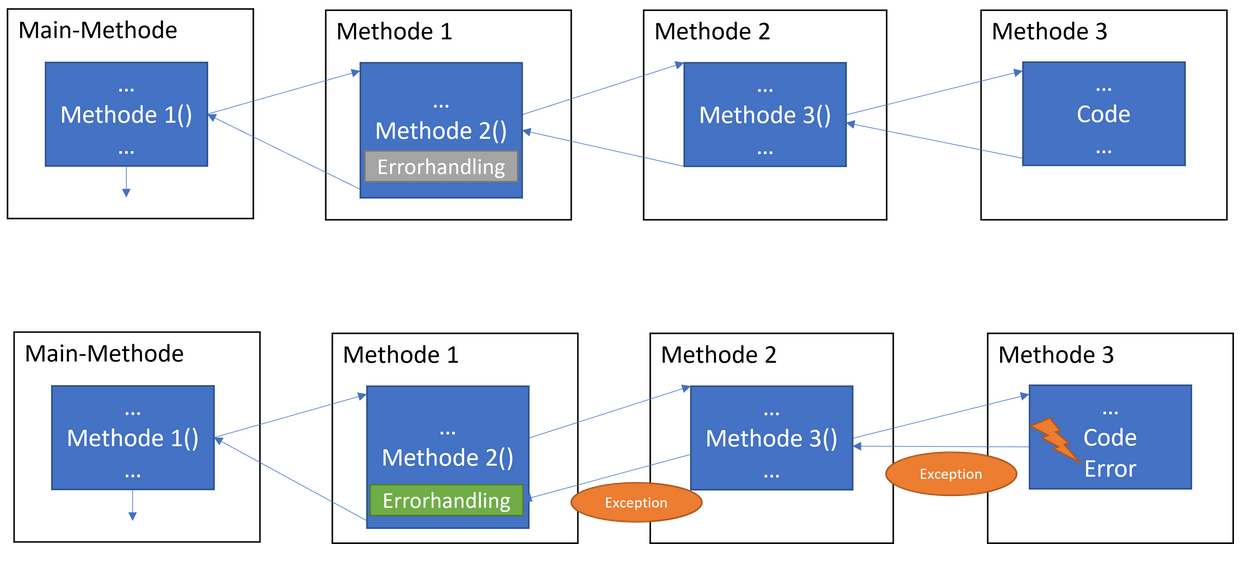
\includegraphics[width=1\textwidth]{pics/fehlerBehandlung.png}

    Exceptions sind einfach Klasse die von der Klasse Exceptions erben. 
    Java stellt uns schon ein paar Exceptions zu verfügung aber, falls wir selber eine ausgabe 
    definieren wollen könne wird das z.b so mache:

    \begin{lstlisting}
class MyException extends Exception {
    MyException(String errorMessage) {
        super(errorMessage);
    }
}
    \end{lstlisting}

    Im Konstruktor müssen wir jeweils den Superklassenkonstruktor (also den Konstruktor der Klasse Exception) aufrufen.
    Dieser nimmt als Argument einen String entgegen, der die Fehlermeldung enthält.

    Wenn eine Fehelr im Code auftritt erstellen wir eine Instanz einer Exceptions 
    und werfen die mit \textbf{throw}

    \begin{lstlisting}
if (unexpectedSituation) {
    MyException myException = new MyException("something unexpected happens");
    throw myException;
}
    \end{lstlisting}

    Wenn eine Methode eine Exception werfen kann, müssen wir das angeben. 
    Die geschieht auch mit dem Wort \textbf{throw}. Dannach führen wir einfach auf, welche Exceptions geworfen werden 
    können. 

    \begin{lstlisting}
void exampleMethod() throws MyException {
    // ...
    if (unexpectedSituation) {
        MyException myException = new MyException("something unexpected happens");
        throw myException;
    }
    // ...
}
    \end{lstlisting}

    Wenn eine Methoden eine wetere Methode aufruft die einen Fehler werfen kann. Müssen wir diesen entweder 
    behandeln oder an den aufrufenden weitergeben. 

    Wenn wir den Fehler behandeln wollen müssen wir ihn Fangen: 

    \subsection*{Try catch}

    \begin{lstlisting}
try { // Start des geschuetzten Bereichts
    // ...
    exampleMethod() // hier kuennte ein Fehler auftreten
    // ...
} catch (Exception e) {
    // Fehlerbehandlung
}
    \end{lstlisting}

    Die Methode, welche einen Fehelr wefen kann, wird mit einem \textbf{try}-block umfasst und 
    im \textbf{catch}-block wird der Feheler behandelt indem auf die Variable e zugegriffen werden kann. 

    \subsection*{finally Klausel}

    Die finally Klausel wird immer ausgeführt und ist dazu da um dinge aus zu führen die 
    in einem Fehlerfall wie auch sonst passieren müssen. z.b wenn dateien erzeug wurde die wieder 
    gelöscht werden müssen. 
    Java garantier sogar das asus führen der finally-klausel auch wenn im catch-block wieder ein Fehler aufgetreten ist. 

    \begin{lstlisting}
try { // Start des geschuetzten Bereichts
    // ...
    exampleMethod() // hier koennte ein Fehler auftreten
    // ...
} catch (Exception e) {
    // Fehlerbehandlung
} finally {
    // Code der immer ausgefuehrt werden muss
}
    \end{lstlisting}

    \textbf{RuntimeExceptions} könne immer auftreten weshalb sie nicht und die von ihnen 
    abgeführten Fehler nicht deklariert werden müssen. 

    \subsection*{Optionals}

    Es gibt Situationen in welchen eine Fehler zu erwarten ist. 

    \begin{lstlisting}
class Employees {
    public Employee getEmployeeWithId(int id) { /* ...*/  }
}
    \end{lstlisting}

    Falls es keinen angestellten mit der ID gibt, gibt es einen Fehler. 
    Dies ist zu erwarten und wir könnten einen Fehler werfen. 
    Da dies aber zu erwarten ist, sollte das mit der "normalen" Pogrammierlogik gelöst 
    werden. 

    Wir könnten null zurück geben, fall der angestellten nicht existiert. Das
    hat aber viele Probleme. Einerseits erkennen wir das an der methode nicht das
    ein Feheler auftreten kann und mit \textbf{null} könne wir nicht viel anfangen. 

    Die Klasse \textbf{Optional} gibt uns eine bessere Lösung. 
    \href{https://docs.oracle.com/en/java/javase/17/docs/api/java.base/java/util/Optional.html}{Die ganze Klasse}
    Eine grobe Definition der klasse: 

    \begin{lstlisting}
class Optional<T> {
    T value = null;

    private Optional(T value) {
        this.value = value;
    }
    static <T> Optional<T> of(T value) { 
        return new Optional<T>(value);
    }

    static <T> Optional<T> empty() { 
        return new Optional<T>(null);
    }

    boolean isPresent() { 
        return this.value != null;
    }

    public T get() {
        if (value == null) {
            throw new NoSuchElementException("No value present");
        }
        return value;
    }
}
    \end{lstlisting}

    Wir sehen, dass ein Optional entweder durch die Methode Optional.empty() oder Optional.of() kreiert werden kann. 
    Im ersten Fall wird ein Optional erzeugt, dass keinen Wert enthält, im zweiten Fall wird der übergebene Wert gespeichert. 
    Mittels der isPresent Methode kann abgefragt werden, ob das Optional einen Wert enthält. 
    Die get Methode wird benutzt, um den Wert zu erhalten

    \begin{lstlisting}
class Employees {
    public Optional<Employee> getEmployeeWithId(int id) { /* ...*/  }
}

int id = 5;
Optional<Employee> maybeAnEmployee = employees.getEmployeeWithId(id);
if (maybeAnEmployee.isPresent()) {
    Employee employee = maybeAnEmployee.get()
   // Normale Programmlogik
} else {
   // Logik fuer den Fall, dass Employee nicht gefunden wurde. 
}
    \end{lstlisting}

    Diese Lösung hat grosse Vorteile. Erstens sehen wir an der Methodensignatur Optional<Employee> getEmployeeWithId(int id), dass diese Methode eventuell keinen Wert zurückliefert. 
    Zudem können wir die Fehlerbehandlung gar nicht versehentlich vergessen, da wir ja nicht direkt auf den Wert employee zugreifen können, ohne zuerst get() aufzurufen. 
    Der Java-Compiler wird uns anderenfalls eine Fehlermeldung geben, und uns daran erinnern, dass wir noch eine Fehlerbehandlung machen sollten.

    \section*{Funktionales Programmieren}
    
    Funktionales Programmieren ist eine andere Art der Programmierlogik, im vergleich zum Objektorientierten Programmieren. 
    Beim Funktionale Programmieren werden funktionen im mathematischen sinne betrachtet. 
    $f : I \rightarrow  O$ Wenn wir eine eingabe machen krigen wir einen neuen Wert herraus. 

    Nehmen wir an wir haben eine funktion $f : I \rightarrow R$  und eine funktion $g: R \rightarrow O$. So könne wir ein 
    grösseres programm $h(x)$ schreiben. 

    $$ h: I \rightarrow O $$
    $$ h(x) = g(f(x))$$

    Ein konretes Beispiel: 

    \begin{lstlisting}
class FunctionalTest {
    static double square(double x) {
        return x * x;
    }

    static int round(double number) { 
        return (int) (number + 0.5);
    }

    static int roundSquared(double x)  {
        return round(square(x));
    }
}
    \end{lstlisting}

    Diese Hintereinanderausführung von Funktionen klingt zuerst einmal nicht besonders spannend. 
    Ein weiteres Element, welches die funktionale Programmierung sehr mächtig macht, ist, dass darin Funktionen einfach Werte sind. 
    Damit können diese zum Beispiel als Parameter an andere Funktionen (Methoden) übergeben werden. Oder sie können als Rückgabewert aus einer Methode zurückgegeben werden. 
    Wie wir noch sehen werden, macht es dies möglich, gewisse Arten von Berechnungen sehr elegant und verständlich auszudrücken.

    Ein weiteres Merkmal von diesem Programmierstil ist, dass Daten von einer Funktion nicht verändert werden. 
    In der objektorientierten Programmierung wird oft das Verändern von Daten nur von Methoden eines Objektes erlaubt. 
    Im Gegensatz dazu wird es in der funktionalen Programmierung gänzlich vermieden. Stattdessen werden die Eingabedaten einer Funktion wenn nötig kopiert, und nur diese Kopie wird verändert. 
    Dies macht das Verstehen von Programmen einfacher, da wir nicht im Kopf Buch führen müssen, welche Daten von welcher Funktion verändert wurden.

    \subsection*{Funktionsobjekte}

    Eine Zentrale idee des funktionalen Programmierens ist, das Funktionen Werte sind. Funktionen könne also 
    als Variabeln gespeichert werden und so auch als Parameter anderen Funktione übergeben und auch aus Funktionen 
    zurück gegeben werden. 
    In Java simulieren wir dies indem wir Funktionen als Objekte repräsentieren. 

    \begin{lstlisting}[caption=funktion]
interface Function<T, R> {
    R apply(T x);
}
    \end{lstlisting}

    Dieses Interface bildet eine Funktion $f: R \rightarrow T$. T ist der eingabewert und R der Rückgabewert. 

    So könnte wir die methode \textbf{square} implementieren. 

    \begin{lstlisting}[caption=square als Funktion]
class SquareFunction implements Function<Integer, Integer> {
    public Integer apply(Integer x) {
        return x * x;
    }
}
    \end{lstlisting}
    
    Objekte dieser Funktionen können nun an Methoden übergeben werden:

    \begin{lstlisting}
class FunTest {
    static int valueAtX (Function<Integer, Integer> fun, Integer x) {
        return fun.apply(x);
    }

    public static void main(String[] args) {
        int squareOf2 = valueAtX(new SquareFunction(), 2);
        int cubeOf2 = valueAtX(new CubicFunction(), 2);
    }
}
    \end{lstlisting}

    \begin{lstlisting}[caption=square und cube als funktion]
    interface Function<T, R> {
    R apply(T x);
}

class PowerFunction implements Function<Integer, Integer> {
    int n = 0;

    public PowerFunction(int n) {
        this.n = n;
    }

    public Integer apply(Integer x) {
        int pow = 1;
        for (int i = 0; i < n; i = i + 1) {
            pow = pow * x;
        }
        return pow;
    }
}

class Main {
   static int valueAtX (Function<Integer, Integer> fun, Integer x) {
        return fun.apply(x);
    }
    
    static Function<Integer, Integer> nthPower(int n) { 
      return new PowerFunction(n);
      
    }
  
  public static void main(String[] args) {
    Function<Integer, Integer> squareFunction = nthPower(2); 
    Function<Integer, Integer> cubicFunction = nthPower(3);
    
    System.out.println("square at 2: " + valueAtX(squareFunction, 2));
    System.out.println("cube at 2: " + valueAtX(cubicFunction, 2));
  }
}}
    \end{lstlisting}

    \subsection*{Lambda-Ausdrücke und Methodenreferenzen}

    Im \textbf{java.util.function} package ist dieses Interface enthalten, welche eine Funktion simuliert:

    \begin{lstlisting}
interface Function<T, R> {
    R apply(T x);
}
    \end{lstlisting}

    So würden wir mit dem Interface \textbf{Function} eine Funktion definieren:

    \begin{lstlisting}
class SquareFunction implements Function<Integer, Integer> {
    public Integer apply(Integer value) {
        return x * x;
    }
}

Function<Integer, Integer> squareFun = new SquareFunction();
    \end{lstlisting}

    Das alles könne wir mir Lambda-Ausdrücken auf ein Zeile schreiben. 

    \begin{lstlisting}
Function<Integer, Integer> squareFun = (Integer x) -> { return x * x };
    \end{lstlisting}

    Allgemeiner fomuliert entspricht der lambda-asudruck \textbf{(T value) -> {Ausdruck}}:

    \begin{lstlisting}
class LambdaExpression implements Function<Integer, Integer> {
    public R apply(T value) {
        AUSDRUCK;
    }
}
    \end{lstlisting}

    Vieles könne wir an diesem Ausdruck noch verreinfachen. Wir können 
    die Datentypen, die Klammern und das \textbf{return} weglassen. 
    Dann sieht das so aus: 

    \begin{lstlisting}
Function<Integer, Integer> squareFun = x -> x * x;
    \end{lstlisting}

    Es ist auch möglich zwei argumente für eine Funktion zu verwenden. 
    Das Interface dafür heisst \textbf{BiFunction}: 

    \begin{lstlisting}
interface BiFunction<T, U, R> {
    R apply(T x, U y);
}
    \end{lstlisting}

    Und wird so ausgeführt
    \begin{lstlisting}
BiFunction<Integer, Integer, Integer> plusFun = (Integer a, Integer b) -> a + b;
    \end{lstlisting}


    \subsection*{Methodenreferenzen}

    Neben Lambda-Ausdrücken können auch Methoden mit der richtigen Signatur als Wert behandelt werden. 
    Eine Methode mit nur einem Argument könnte also einer Variable mit Typ Function<T, R> zugewiesen werden. 
    Analog dazu können wir eine Methode mit zwei Argumenten einer Variable mit Typ BiFunction<T, U, R> zuweisen. 
    Um die Methode als Wert zu behandeln, schreiben wir den Objektnamen, gefolgt von :: und dem Methodennamen. 
    Dies ist im Folgenden illustriert:


    \begin{lstlisting}
class MethodExample {
    Integer square(Integer x) { 
        return x * x;
    }
    
    public static void main(String[] args) {
        MethodeExample instance = new MethodeExample();

        Function<Integer, Integer> squareFun = instance::square;
    }
}
    \end{lstlisting}

    Und das ganze noch mit Klassen

    \begin{lstlisting}
class MethodExample {
    static Integer square(Integer x) { 
        return x * x;
    }
    
    public static void main(String[] args) {        

        Function<Integer, Integer> squareFun = MethodeExample::square;
    }
}
    \end{lstlisting}

    Und insgesamt:

    \begin{lstlisting}
import java.util.function.Function;


class MethodExample {
    Integer square(Integer x) { 
        return x * x;
    }
    
    static Integer squareStatic(Integer x) { 
        return x * x;
    }
    
}

public class Main {
    public static void main(String[] args) {
        MethodExample instance = new MethodExample();

        Function<Integer, Integer> squareFun = instance::square;
        
        System.out.println(squareFun.apply(7)); //gibt 49
        
        
        Function<Integer, Integer> squareFun2 = MethodExample::squareStatic;
        
        System.out.println(squareFun2.apply(7)); // gibt 49


    }
}
    \end{lstlisting}
\end{document}
